\documentclass[crop,tikz,convert=pdf2svg,border=5mm]{standalone}


% Tikz settings optimized for causal graphs.
\usetikzlibrary{shapes,decorations,arrows,calc,arrows.meta,fit,positioning}
%\usepackage{helvet}
\tikzset{every picture/.style={/utils/exec={\sffamily}}}
\tikzset{
	-Latex,auto,node distance =1 cm and 1 cm,semithick , shorten >=1pt,shorten <=1pt,
}

\begin{document}
	
	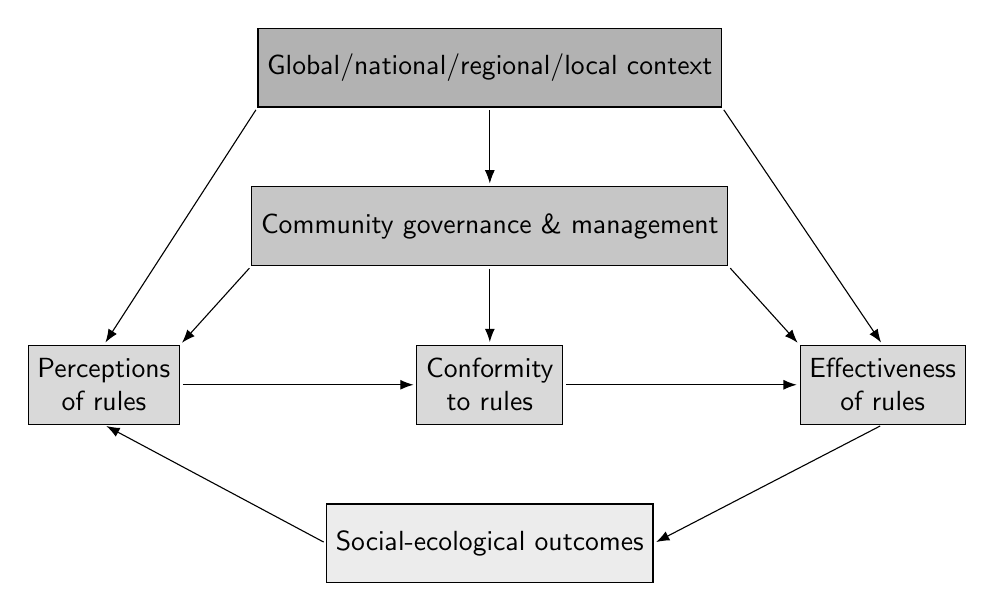
\begin{tikzpicture}[
	node distance =1 cm and 1 cm, 
	state/.style={, draw, minimum size=1cm, rounded corners=0cm},
	stateg1/.style={, draw, minimum size=1cm,fill = gray!60, rounded corners=0cm},
	stateg2/.style={, draw, minimum size=1cm,fill = gray!45, rounded corners=0cm},
	stateg3/.style={, draw, minimum size=1cm,fill = gray!30, rounded corners=0cm},
	stateg4/.style={, draw, minimum size=1cm,fill = gray!15, rounded corners=0cm},
	]
	
	%context
	\node[stateg1, align=center] (1) [] {Global/national/regional/local context};
	%govmgmt
	\node[stateg2, align=center] (2) [below = of 1] {Community governance \& management};
	%rules
	\node[stateg3, align=center] (3) [below = of 2] {Conformity\\to rules};
	\node[stateg3, align=center] (4) [left = of 3,xshift = -2cm] {Perceptions\\of rules};
	\node[stateg3, align=center] (5) [right = of 3, xshift = 2cm] {Effectiveness\\of rules};
	%outcomes
	\node[stateg4, align=center] (6) [below = of 3] {Social-ecological outcomes};
	
	%straight paths
	\path (1.south) edge[] node[above] {} (2.north);
	\path (1.south west) edge[] node[above] {} (4.north);
	\path (1.south east) edge[] node[above] {} (5.north);
	\path (2.south) edge[] node[above] {} (3.north);
	\path (2.south west) edge[] node[above] {} (4.north east);
	\path (2.south east) edge[] node[above] {} (5.north west);
	\path (4.east) edge[] node[above] {} (3.west);
	\path (3.east) edge[] node[above] {} (5.west);
	\path (5.south) edge[] node[above] {} (6.east);
	\path (6.west) edge[] node[above] {} (4.south);

	%label figure if want
	%\node[above = of 7, xshift = -1cm, yshift = 4.5cm] {\large\textbf{A}};
	%\node[above = of 7, xshift = -1cm, yshift = -0.5cm] {\large\textbf{B}};

	\end{tikzpicture}
	
\end{document}


